%%%%%%%%%%%%%%%%%%%%%%%%%%%%%%%%%%%%%%%%%%%%%%%%%%%%%%%%%%%%
% 创建时间: Wednesday, April 29, 2026
% 创作者: SHUSHU
% --------------------
% 最后修改时间: 
% 修改者: SHUSHU
% ----------------------------------------
% MIT License
% 
% Copyright (c) 2026 SHUSHU
% 
% Permission is hereby granted, free of charge, to any person obtaining a copy of
% this software and associated documentation files (the "Software"), to deal in
% the Software without restriction, including without limitation the rights to
% use, copy, modify, merge, publish, distribute, sublicense, and/or sell copies
% of the Software, and to permit persons to whom the Software is furnished to do
% so, subject to the following conditions:
% 
% The above copyright notice and this permission notice shall be included in all
% copies or substantial portions of the Software.
% 
% THE SOFTWARE IS PROVIDED "AS IS", WITHOUT WARRANTY OF ANY KIND, EXPRESS OR
% IMPLIED, INCLUDING BUT NOT LIMITED TO THE WARRANTIES OF MERCHANTABILITY,
% FITNESS FOR A PARTICULAR PURPOSE AND NONINFRINGEMENT. IN NO EVENT SHALL THE
% AUTHORS OR COPYRIGHT HOLDERS BE LIABLE FOR ANY CLAIM, DAMAGES OR OTHER
% LIABILITY, WHETHER IN AN ACTION OF CONTRACT, TORT OR OTHERWISE, ARISING FROM,
% OUT OF OR IN CONNECTION WITH THE SOFTWARE OR THE USE OR OTHER DEALINGS IN THE
% SOFTWARE.
% ----------------------------------------
% 更改日志:
% 日期       	说明
% -----------	------------------------------------
%
%  长春大学毕业论文模板 — 完整功能演示
%
%  本文件演示了模板支持的全部特性：
%    - 封面 / 中英文摘要 / 目录
%    - 多级标题 (chapter/section/subsection)
%    - 图片 (单图、子图、TikZ 矢量图)
%    - 三线表格
%    - 数学公式 (行内、行间、矩阵、多行对齐、分段函数)
%    - 代码块
%    - 列表 (有序/无序)
%    - 交叉引用
%    - 参考文献引用与自动编号
%    - 致谢
%
%  编译: xelatex → bibtex → xelatex × 2
%%%%%%%%%%%%%%%%%%%%%%%%%%%%%%%%%%%%%%%%%%%%%%%%%%%%%%%%%%%%

% !TeX program = xelatex
\documentclass{ccu_thesis}

% --- 基本信息填写 ---
\title{设计题目}
\entitle{English Thesis Title}
\author{XXX}
\studentid{XXXXXXXXX}
\academy{XXX学院}
\department{XXX} % 建议填写具体专业
\Class{XXXXX班}
\instructor{XXX（职称）}

% 设置封面日期，如果不设置则默认显示当前系统时间
%\thesistime{2025}{5}{25}

\begin{document}

% 渲染封面
\maketitle

% --- 中文摘要 ---
\begin{cnabstract}{虚拟现实；沉浸性；审美沉浸}
以浓缩的形式概括研究课题的主要内容、方法和观点。中文摘要一般要求300～500字。
中文摘要和外文摘要均要求独立成页。
\end{cnabstract}

% --- 英文摘要 ---
\begin{enabstract}{Six-wheeled trolley; Unmanned; Motor control}
The abstract should be consistent with the Chinese version. It should be written in Times New Roman, size 12pt (Xiao Si).
Each keywords should be capitalized.
\end{enabstract}

% 生成目录
\makecontents

% ============= 正文开始 =============

\chapter{绪论}
\section{研究背景与意义}
此处输入正文内容。宋体小四号字，行距固定值 20 磅，首行缩进 2 字符。正文主体是论文中最重要的部分，整个论证过程在此展开。应该结构合理、层次清晰、重点突出、文字简练、通顺。

\section{国内外研究现状}
二级标题段前段后各空一行（约20bp）。

\chapter{排版示例与功能测试}
这是小四号的正文字体，段间距由类文件统一控制。
通过空一行实现段落换行，仅仅是回车并不会产生新的段落。
\par 也可以通过\verb|\par|命令来新起一段。

\section{多级标题测试}
\subsection{二级小节样式}
\subsubsection{三级小小节样式}
这是三级标题下的内容。
\subsection{另一小节}
\subsubsection{三级小标题测试}\label{subsubsubsec:test}

\paragraph{段落标题}\label{para:para}这是一个带有顶头标签的段落。这是一个带有顶头标签的段落。这是一个带有顶头标签的段落。

\section{字体效果测试}
本模板已经引入伪加粗和伪斜体：
{\songti \bfseries 宋体加粗}，{\songti \itshape 宋体斜体}，{\songti \bfseries \itshape 宋体粗斜体}。

请注意，使用加粗和斜体时，建议与字体名称一同使用，否则会自动匹配为黑体或楷体：
{\bfseries 纯加粗变黑体}，{\itshape 纯斜体变楷体}。

\chapter{参考文献与公式引用}\label{ch:ref}
\section{参考文献引用示例}\label{sec:bibs}
这是一个参考文献引用的范例\cite{Stone_1998}，你可以随时使用两种不同的样式\cite{Stone_1998}或者上标样式\upcite{Stone_1998}。
可以同时引用多个文献\cite{Stone_1998,9780124467422,huagongrenzheng2014}。

\subsection{交叉引用测试}\label{subsec:crossref}
使用\verb|\autoref|命令引用：\autoref{ch:ref}、\autoref{sec:bibs}和\autoref{subsec:crossref}。
以及引用之前的段落：\nameref{para:para}。

\section{数学公式环境示例}
在文中引用公式可以这么写：$a^2+b^2=c^2$。
\begin{equation}
	\sin^2{\theta}+\cos^2{\theta}=1 \label{eq:pingfanghe}
\end{equation}
引用如式~\eqref{eq:pingfanghe}~或者\autoref{eq:pingfanghe}。

下面是矩阵测试（使用了 \verb|\bm| 宏包）：
\begin{equation}
	\bm{A}=\begin{bmatrix}
		1  & 2  & 3  & 4  \\
		11 & 22 & 33 & 44 \\
	\end{bmatrix}
	\times\begin{bmatrix}
		22 & 24 \\
		32 & 34 \\
		42 & 44 \\
		52 & 54 \\
	\end{bmatrix}
\end{equation}

下面是 Cauchy 不等式测试（使用了 \verb|\leqslant|）：
\begin{equation}
	\left(\int_{E}|f(x) g(x)| \mathrm{d} \mu\right)^{2} \leqslant \int_{E}|f(x)|^{2} \mathrm{d} \mu \int_{E}|g(x)|^{2} \mathrm{d} \mu
\end{equation}

\chapter{代码、图表与复杂图例}

\section{代码块演示}
\begin{lstlisting}[language=Python, caption={Python 打印示例}]
print('hello world')
\end{lstlisting}

\begin{lstlisting}[language=C++, caption={C++ 结构体示例}]
struct node {
    int cnt;
    node *next[26], *fail;
    node() { cnt=0; fail=NULL; }
};
\end{lstlisting}

\section{图表示例}
% 图：图名在下，编号 2.1
\begin{generalfig}{行星轮式爬楼梯轮椅}{fig:wheel}
    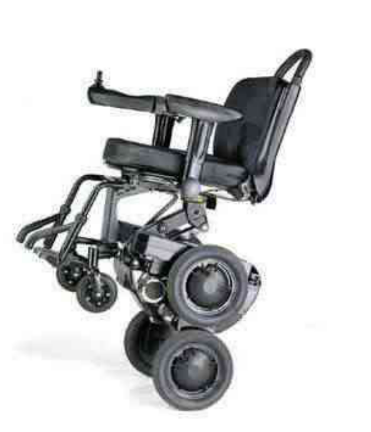
\includegraphics[width=0.5\textwidth]{Figures/1.1.png}
\end{generalfig}
根据\autoref{fig:wheel}所示，该机构设计合理。

\section{表格示例}
\begin{generaltab}[H]{电动爬楼梯轮椅升降机构优缺点对照表}{tab:comparison}
    \begin{tabular}{lccc}
        \toprule
        爬升机构 & 星轮式 & 履带式 & 腿足式 \\
        \midrule
        台阶适应能力   & 一般   & 强     & 强     \\
        稳定性         & 一般   & 强     & 差     \\
        控制难易       & 易     & 一般   & 难     \\
        \bottomrule
    \end{tabular}
\end{generaltab}

\section{带说明文字的复杂图例}

% 必须使用标准的 figure 环境，以便手动控制 caption 的位置
\begin{figure}[H]
    \centering
    
    % 1. 放置子图图片及 (a) (b) 编号
    \begin{subfigure}[b]{0.4\textwidth}
        \centering
        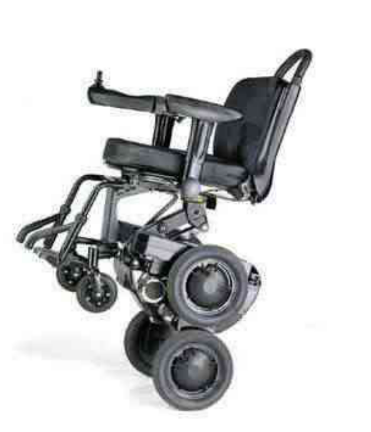
\includegraphics[width=\textwidth]{Figures/1.1.png}
        \caption{} % 自动生成 a) 
    \end{subfigure}
    \hspace{2em}
    \begin{subfigure}[b]{0.4\textwidth}
        \centering
        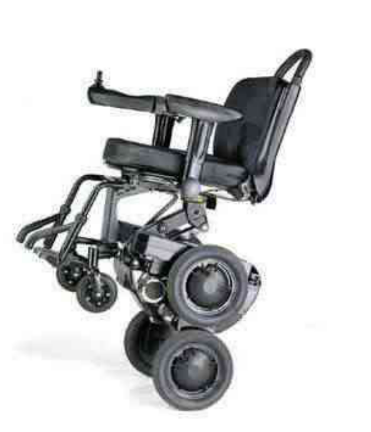
\includegraphics[width=\textwidth]{Figures/1.1.png}
        \caption{} % 自动生成 b)
    \end{subfigure}

    % 2. 放置主图名 (这一行会生成：图 2.1 滑阀式...)
    \caption{滑阀式转向控制阀的结构和工作原理}
    \label{fig:valve_fixed}

    % 3. 在主图名下方放置子图详细名称
    \vspace{0.3em} % 微调主图名与子图名之间的距离
    {\wuhao a) 常流式滑阀 \qquad b) 常压式滑阀} \\
    
    % 4. 放置详细说明文字 (分点)
    \vspace{0.3em}
    {\wuhao 1-阀体 \quad 2-阀套 \quad 3-壳体 \quad 4、6-通动力缸左、右腔的通道}
\end{figure}

% ============= 后置章节 =============

\unnumberedchapter{总结}
结论是围绕本论所作的结束语。基本要点是总括全文，加深题意。

\bibliography{Bibs/mybib}

\unnumberedchapter{致谢}
致谢应以简短的文字对在课题研究过程中给予帮助的人员表示谢意。

\begin{appendices}
    \unnumberedchapter{附录}
    \section{源代码清单}
    附录内容。
    \begin{equation}\label{eq:appendices}
        E = mc^2 
    \end{equation}
\end{appendices}

\end{document}